\documentclass[10pt,oneside]{report}

% Encoding and font packages
\usepackage[table]{xcolor}
\usepackage[utf8]{inputenc}
\usepackage[T1]{fontenc}
\usepackage{lmodern}
\usepackage{booktabs}
\usepackage[nottoc]{tocbibind} % If you don't want the main TOC itself listed
\usepackage{setspace}
\onehalfspacing
\usepackage{hyperref}
\hypersetup{
    colorlinks=true,
    linkcolor=blue,
    filecolor=magenta,      
    urlcolor=cyan,
    citecolor=blue
}
\usepackage[numbers]{natbib}
\usepackage[colorinlistoftodos,prependcaption,textsize=small]{todonotes}
\usepackage{adjustbox}
\usepackage{graphicx}
\graphicspath{ {./images/} }

\usepackage{anyfontsize}
\usepackage{lmodern}
% Dynamically scale font sizes (80% of original)
\let\oldnormalsize\normalsize
\renewcommand{\normalsize}{\fontsize{8}{10}\selectfont}
\let\oldlarge\large
\renewcommand{\large}{\fontsize{10}{12}\selectfont}
\let\oldLarge\Large
\renewcommand{\Large}{\fontsize{11.5}{13.8}\selectfont}
\let\oldLARGE\LARGE
\renewcommand{\LARGE}{\fontsize{13}{15.6}\selectfont}
\let\oldhuge\huge
\renewcommand{\huge}{\fontsize{16}{19.2}\selectfont}
\let\oldHuge\Huge
\renewcommand{\Huge}{\fontsize{20}{24}\selectfont}

% Begin document
\begin{document}

% -------------------------
% Title Page
% -------------------------
\begin{titlepage}
    \centering
    % Title (two lines)
    {\LARGE TODO TITLE\\\par}
    \vspace{2cm}
    % Subtitle/description
    {\large A report submitted to the University of Manchester for the degree of
    Bachelor of Science in the Faculty of Science and Engineering\par}
    \vspace{2cm}
    \vspace{1cm}

    {\large Author: Sai Putravu\par}
    {\large Student id: 10829976\par}
    {\large Supervisor: TODO\par}
    \vfill
    % Department
    % Date
    {\large 2025\par}
    \vspace{1cm}
    {\large School of Computer Science\par}
\end{titlepage}

% Roman page numbering for preliminary pages
\pagenumbering{roman}

% -------------------------
% Table of Contents
% -------------------------
\tableofcontents
\clearpage

% -------------------------
% List of Figures
% -------------------------
\listoffigures
\clearpage

% -------------------------
% List of Tables
% -------------------------
\listoftables
\clearpage


% -------------------------
% Abbreviations and Acronyms
% -------------------------
% \phantomsection
\addcontentsline{toc}{chapter}{Abbreviations and Acronyms}
\chapter*{Abbreviations and Acronyms}

\todo{Alphabetically sort this}
\begin{table}[ht]
    \centering
    \begin{tabular}{ll}

        \textbf{BERT} & Bidirectional Encoder Representation from Transformers. \\
        \textbf{CBM} & Condition-based maintenance policy. \\
        \textbf{CNN} & Convolutional Neural Network. \\
        \textbf{DBSCAN} & Density-Based Spatial Clustering of Application with Noise. \\
        \textbf{DL} & Deep Learning. \\
        \textbf{ELMo} & Embeddings from Language Models. \\
        \textbf{FLD} & First-line diagnosis system. \\
        \textbf{GPT} & Generative Pre-trained Transformer. \\
        \textbf{HDBSCAN} & Hierarchical Density-Based Spatial Clustering of Application with Noise. \\
        \textbf{HDD} & Hard-Disk Drive. \\
        \textbf{IoT} & Internet of Things. \\
        \textbf{LSA} & Latent Semantic Analysis. \\
        \textbf{ML} & Machine Learning. \\
        \textbf{NLP} & Natural Language Processing. \\
        \textbf{PCA} & Principle Component Analysis. \\
        \textbf{PdM} & Predictive maintenance policy. \\
        \textbf{PLM} & Pre-trained Language Model. \\
        \textbf{PvM} & Preventative maintenance policy. \\
        \textbf{R2F} & Run-to-failure maintenance policy. \\
        \textbf{RF} & Random Forest. \\
        \textbf{SAFE} & Supervised Aggregative Feature Extraction. \\
        \textbf{SMART} & Self-monitoring and reporting technology. \\
        \textbf{STFC} & Science and Technology Facilities Council. \\
        \textbf{SVD} & Singular Value Decomposition. \\
        \textbf{SVM} & Support Vector Machine. \\
        \textbf{t-SNE} & t-distributed Stochastic Neighbour Embedding. \\
        \textbf{UMAP} & Uniform Manifold Approximation and Projection. \\

    \end{tabular}
\end{table}

\clearpage

% Switch to Arabic numbering after preliminary pages
\pagenumbering{arabic}

% -------------------------
% Chapters
% -------------------------
\chapter*{Abstract}
\todo[inline]{TODO}


\chapter{Introduction}

This project concerns the use of statistical and Machine Learning models to augment the predictive maintenance process at the STFC Rutherford Appleton Laboratory's ISIS Neutron and Muon research facility. The ISIS Neutron and Muon facility is a research centre for physical and life sciences, owned and operated by the STFC, a council that forms the UK Research and Innovation. In order to produce beams of neutrons and muons, allowing scientists to study materials at the atomic level, large and complex structures and machinery are required. The facility has a wealth of instrumentation taking multitudes of measurements to ensure that proper maintenance is completed in a timely manner. \\

\todo[inline] {Finish this off}
\textbf{ }
\todo[inline,caption={}]{
Introduce the sections of the paper.
\begin{itemize}
    \item Refine this after coming back
    \item Section 2,
    \item Section 3, 
    \item ...
\end{itemize}
}


\section{Motivation}
Motivate the research project.


\todo[inline,caption={}]{
The things in this section will include
\begin{itemize}
    \item Introduce the problem: Auto-categorisation and label inference
    \item Highlight the research aims. This should highlight the vastly open nature of the project and then hone in on the particular issue I am tackling. (i.e. to progress the state of PdM ...)
    \item Identify the data input, expected output, data shape and explain why this motivates the project
\end{itemize}
}

\chapter{Background}
\todo[inline,caption={}]{
The things in this section will include
\begin{itemize}
    \item Background
    \item Literature Review
    \item Looking at general predictive maintenance 
    \item Looking at general predictive maintenance in industrial applications
    \item Similar pairwise sentence similarity literature
    \item Similar literature in text clustering
    \item Similar literature in specifically sentence clustering in industrial applications
\end{itemize}
}
\section{Overview of the ISIS Research Facility}

\todo[inline,caption={}]{
Introduce the research topic. 
The things in this section will include
\begin{itemize}
    \item Talk about the ISIS research facility
    \item Talk about the Operational Cycle for ISIS (graph too)
    \item Talk about the ISIS Crew and importance of having trained staff on premises.
    \item Talk about the Lost time and why it is important to minimise this for the ISIS research facility.
    \item Describe the first-line diagnosis system (FLD) and FAPs.
    \item Talk about the Datasets, operalog
\end{itemize}
}


\section{Maintenance Techniques}
In industry, the uptime of production systems are strongly coupled with the equipment maintenance. So much so that what was once considered a `necessary evil' is now seen as a `profit contributor' to be able to maintain a competitive edge \cite{waeyenbergh2002framework, faccio2014industrial}. For facilities aiming to provide systems for research, maintenance impacts the downtime and cost of running. As a result, both to minimise unexpected downtime and provide a competitive edge, many industrial applications collect vast quantities of data during the entire life cycle of the system. This large amount of data may include information about processes, events and alarms \cite{carvalho2019systematic} which occur along the industrial production line, collected by different equipment. The equipment may be located in different locations in the sub-components of the larger system or even different sub-components themselves. \todo{talk about maintenance itself in a lot more depth}

In the literature, various terms and categories of maintenance arise each with differing strategies \cite{susto2012predictive, mobley2002introduction, susto2016dealing}. Thus, while there exists some disagreement in nomenclature, we consider the four categories presented in (\citet{susto2012predictive}). The four maintenance policy categories are as follows, noting that each policy has, uniquely, their own benefits and drawbacks:

\begin{enumerate}
    \item{Run-to-failure (R2F) maintenance: Continual usage of the system until failure. Restoration is performed at the point of noticing failure condition. This is the simplest approach and typically the most costly method as it reduces the facility's availability and requires a complete replacement of parts.} 
    \item{Preventative maintenance (PvM): Otherwise referred to as scheduled maintenance, performing maintenance at regular intervals to increase longevity of the component or in anticipation of the end of expected life of the component. While this typically prevents many errors, it wastes maintenance cycles when systems are perfectly healthy. Hence, causing unnecessary downtime and cost.}
    \item{Condition-based maintenance (CBM): Taking the action to perform maintenance on equipment through monitoring various health characteristics and metrics of the components of the system. This approach requires continuous monitoring and, thus, allows for close to instant response on maintenance only when required. However, a drawback of this policy is that one cannot plan maintenances in advance.}
    \item{Predictive maintenance (PdM): Otherwise referred to as statistical-based maintenance, only performs maintenance actions when determined necessary. Prediction tools are utilised to implement forward-planning and scheduling systems, using statistical inference methods. However, if these statistical inferences are not accurate, the whole system suffers which inevitably leads to additional downtime and costs.}
\end{enumerate}
It should be noted, that several sources conflate CBM and PdM \cite{mobley2002introduction}. As in (\citet{susto2012predictive}), where they are given as separate categories, we follow suit. \\ 

The PdM strategy stands out in the four categories presented as, given a statistical inference model that is able to detect faults accurately, this policy optimises the trade-off between improving equipment condition, reduce failure rates for equipment and minimising maintenance costs \cite{carvalho2019systematic}. This technique enables one to apply foresight for pre-emptive scheduling of large-scale maintenance. \todo{Implement the ISIS version of this in the background. Talk about the FIRST LINE DIAGNOSIS system} As pointed out in Section~(\todo{fill this}...), the ISIS facility aims to strike a balance between PvM, CBM and PdM through periods of large-scaled scheduled maintenance and collection of high quantities of metrics. This is done through the careful coordination between cycle scheduling, day-to-day crew-based monitoring and the FLD \cite{thomason2019isis}.

In industry, many maintenance strategies prefer using PdM whilst experimenting with a variety of statistical inference and artificial intelligence modelling approaches \cite{mobley2002introduction, jezzini2013effects}. Some examples from \cite{carvalho2019systematic} are listed in Table~\ref{tab:pdmPaperTable} which highlights the trend in the industry towards more accurate, ML-based approaches.

\rowcolors{2}{gray!10}{white}
\begin{table}[htbp]
    \fontsize{8}{12}\selectfont
    \centering
    \caption{\fontsize{9}{10}\selectfont Examples of applications of PdM for industrial maintenance strategies.}
    \label{tab:pdmPaperTable}
    \begin{adjustbox}{max width=\textwidth}
    \begin{tabular}{p{1.5cm} p{8.5cm} p{3cm}}
        \toprule
        \textbf{Type} & \textbf{Description} & \textbf{Reference} \\
        \midrule
        Statistical & Application of SAFE to deal with PdM problems characterised by time-series data. The approach is tested on a real-life dataset of the semiconductor ion implantation process. & (\citet{susto2016dealing})\\
        ML & Application of SVM classification for fault prediction of rail networks, with discussion on using the model in optimising trade-offs related to maintenance schedule and costs. & (\citet{li2014improving})\\
        ML & Audio analysis on IoT devices, enabling acoustic event recognition for machine diagnosis. This paper describes designing an end-to-end system, utilising CNN-based classification. & (\citet{pan2017cognitive})  \\
        ML & Utilisation of RF decision trees trained on SMART data to predict reliability of HDD in real-time. & (\citet{su2018real}) \\
        \bottomrule
    \end{tabular}
    \end{adjustbox}
\end{table}


\section{Sentence Similarity}\label{sec:sentenceSimilarity}
\todo{Think of a good transition between PdM and Doc Similarity}

Sentence similarity, otherwise referred to as document similarity, is the (NLP) task of computing the quantification of the similarities between two sentences, documents or texts. This task is motivated by the increasingly large amount of digitisation of human languages (and data, in general), calling for the need to understand similarity between various texts \cite{raju2022sentence}. Examples of the use-cases of sentence similarity include: detection of academic malpractice via plagiarism \cite{lukashenko2007computer, baba2017plagiarism} and text summarisation \cite {aliguliyev2009new, kumar2020semantic, jo2017k}. According to \cite{raju2022sentence}, there are two main types of sentence similarities: (1) lexical similarity and (2) semantic similarity. The former is a computation of the equality between the lexicon of two sentences (i.e. a purely syntactical view), as opposed to the latter  being a comparison between the semantics. Further, the type we focus on, semantic similarity can be split into three types: 

\begin{itemize}
    \item String-based similarity: Measures similarity directly between two strings, accounting for string sequences and character composition. These can be fine-grained, i.e. character-based; coarse-grained, i.e. term-based; or a hybrid mixture of both \cite{yu2016string}.
    \item Knowledge-based similarity: Measures the degree to which two sentences are related, utilising semantic networks (i.e. knowledge graphs). Examples of Knowledge-based similarity approaches include WordNet \cite{budanitsky2001semantic}, the most popular type of approach.
    \item Corpus-based similarity: Premised on a provided corpus, a large database of text to derive inferences from. Methods of this type require the development statistical or DL models that train on the provided corpus and estimate the similarity between two sentence-pair inputs. Popular examples include traditional statistical models, such as LSA \cite{landauer1998introduction} and SVD \cite{steinberger2005text} as well as word embedding models (utilising ML), such as Word2Vec \cite{bojanowski2017enriching}, GloVe \cite{pennington2014glove} and fastText \cite{mikolov2013efficient}.
\end{itemize}

Most of the models mentioned above require some numerical representation of the text to be able to apply mathematical procedures for similarity calculation. Computing this representation involves converting unstructured textual data into one or more vectors. Typically, this process includes (1) general pre-processing steps such as stop-word removal, case normalisation, parts-of-speech tagging, lemmatisation, and tokenisation \cite{tabassum2020survey}; and (2) applying an embedding model, either to a single token (word embedding) or to a sequence of tokens (sentence embedding). Step (1) can be seen as a feature extraction step applied on the unstructured textual data, where feature extraction is the process of extracting the most useful components of the data \cite{sammons2016edison}. For example, part-of-speech tagging can be seen as introducing non-trivial features to some token through extracting the surrounding context. 

This representation is known as an embedding, with the span of the possible vectors referred to as the embedding space. The dimension of the span is termed the embedding dimension. This is an important concept because the characteristics of the embedding space influence the model's ability to capture syntactic and semantic meaning in text, as the embedding space itself encodes this information. This can be seen in the Word2Vec model, described in (\citet{bojanowski2017enriching}), which shows different embedding dimensions produce different results. Another conclusion that can be drawn from this paper is that, if embedding space is not constructed to maximise the meaning of texts, the accuracy of model predictions tends to deteriorate. 

Therefore, the problem of sentence similarity can be directly mapped from the problem of sentence embedding (otherwise referred to as text embedding), where text embedding is the (NLP) task of learning a high-dimensional embedding space representation. Various aspects of text embedding are more thoroughly covered in Section~\ref{sec:sentenceEmbedding}. However, with the advent of the transformer architecture \cite{vaswani2017attention} and rise of the large language models, text embedding has been increasingly solved using DL models with high parameter counts \cite{cao2024recent} and considering extremely large token sequences. Nowadays, word embedding models are considered obsolete with (\citet{cao2024recent}) only considering these models second-generation. Further, the paper states newer generations fall into the following categories:
\begin{itemize}
    \item Third-generation: contextualised embeddings. These models dynamically account for contexts, encoding them into the embedding space. Examples of models include ELMo \cite{sarzynska2021detecting}, GPT \cite{radford2018improving} and BERT \cite{devlin2019bert}. As these models are trained to both understand some embedding space and generate natural language text, they are canonically referred to as language models.
    \item Fourth-generation: universal text embeddings. The generation which is currently state-of-the-art, with the aim of developing a unified model which is able to address multiple downstream tasks. Examples of models in this generation, making progress towards unification include Gecko \cite{lee2024gecko}, Multilingual e5 text embeddings \cite{wang2024multilingual}, Nomic \cite{nussbaum2024nomic} and many more. 
\end{itemize}

Second-, third- and fourth-generation text embedding models are used frequently in PdM for applications such as insight extraction \cite{abijith2023large,usuga2022using} and clustering intents from unstructured text data \cite{nota2022text}. Sources of natural language datasets, in industrial applications typically arise from operational or managerial log files which document aspects such as failures, resolutions and comments similar to the ISIS facility failure logs \todo{cite and fill when section exists}(\cite{todo} see Section~\ref{}). Advanced text embedding models enable for semi- or fully automatic insight retrieval and auto-categorisation, enabling intuitive understanding of the textual datasets potentially highlighting patterns in failure.


\section{(maybe) Clustering}
Talk about clustering lit. rev.
\todo{Think of a good transition between Sentence Similarity and Clustering}
\todo[inline]{Think whether it is useful to present literature review in this section.}

\todo[inline, caption={}] {
The things in this section will include
    \begin{itemize}
        \item (DONE) Looking at general predictive maintenance 
        \item (Done) Looking at general predictive maintenance in industrial applications
        \item (Done) Similar pairwise sentence similarity literature
        \item Similar literature in text clustering
        \item (sort of DONE) Similar literature in specifically sentence clustering in industrial applications
    \end{itemize}
}

\chapter{Natural Language Processing Background}
This chapter delves into the technical background required in understanding and appreciating the approach proposed in Chapter~\ref{chap:Methodology}. Firstly, in Section~\ref{sec:BERT}, we discuss the technical details of the (third-generation text embedding) BERT model and its family of encoder-only transformers \cite{devlin2019bert}. Specifically we further explore two improvements over BERT (XLNet \cite{yang2019xlnet} and MPNet \cite{song2020mpnet}). Then, in Section~\ref{sec:nomic}, we explore the state-of-the-art, fourth-generation Nomic \cite{nussbaum2024nomic} architecture. After, we cover two methods of dimensionality reduction (PCA \cite{pearson1901liii,hotelling1933analysis} and UMAP \cite{mcinnes2018umap}) motivated by the need to visualise samples from the high-dimensional embedding spaces of the aforementioned models, in Section~\ref{sec:dimred}. Finally, we present three clustering algorithms - with one supervised (k-Medoids \cite{}) and two unsupervised (DBSCAN \cite{ester1996density} and HDBSCAN \cite{campello2013density}) in addition to four clustering evaluation metrics. The clustering metrics we look at are: (1) Inertia \todo{find the reference for this}\cite{}, (2) Silhouette \cite{rousseeuw1987silhouettes}, (3) Davies-Bouldin Index \cite{davies1979cluster}, (4) Calinski-Harabasz Index \cite{calinski1974dendrite}. \todo{maybe talk about optuna, if we use it.} \todo{double check all citations here are not empty}\\ 

\todo[inline,caption={}]{
Describe the various technical factors required before attempting to understand the methodology.
The things in this section will include
\begin{itemize}
    \item Discuss sentence embedding, similarity measures: BERT, RoBERTA, MPNet, XLNet, NOMIC.
    \item Dimensional reduction techniques and need for them (UMAP, PCA, t-SNE).
    \item Clustering methods: kmedoids, DBSCAN, DBSCAN*/HDBCAN
    \item Clustering evaluation methods: todo I don't remember these off the top of my head 
    \item Maybe briefly touch on Optuna?
\end{itemize}
}

\section{Sentence Embedding}\label{sec:sentenceEmbedding}
Briefly touched on in Section~\ref{sec:sentenceSimilarity}, sentence embedding (otherwise known as text embedding) is the NLP task of computing some high-dimensional embedding vector-space representation for unstructured text data. This numerical representation should encode the semantic and syntactic meaning of the text and establish meaningful relationships. For example, the sentence `I like dogs' should have the opposite representation to \todo{Maybe add this as an image illustration} `I hate dogs'.  However these sentences should be more related than to the sentence `My house was destroyed in an earthquake'. Deep learning sentence embedding models are now seen to be state-of-the-art as they are able to extract features automatically and more effectively than manual efforts, when supported with large quantities of data \cite{liang2017text}.

\subsection{BERT-family Transformers}\label{sec:BERT}
Pre-trained language models (PLMs), such as BERT \cite{devlin2019bert}, have been widely successful in a wide range of NLP tasks through fine-tuning \cite{edunov2019pre, min2023recent}. Fine-tuning is the process of re-training a PLM on specialised tasks, leveraging the model's base knowledge, by applying perturbations to the pre-trained model parameters through gradient descent learning algorithms. These language models, trained on (1) finding an embedding space for natural language and (2) stochastically generating tokens to mimic natural language, often provide a great platform to perform task-specific model fine-tuning. 
Platforms such as HuggingFace \cite{wolf2019huggingface}, allow authors to upload these pre-trained model parameters which in-turn allows researchers to download them for them fine-tuning. Moreover, task-specific fine-tuned models parameters are uploaded, downloaded and shared on these platforms. These fine-tuned models are useful for researchers whose focus lies outside of optimising these model parameters.
In this section, we talk about the BERT-family of language models.

\subsubsection{BERT}
The Bidirectional Encoder Representations from Transformer (BERT) language model introduced in (\citet{devlin2019bert}) was designed to learn deep bidirectional representations from unlabelled text. It achieved this by learning the left and right context in every layer of the model. The model implementation can be split into two phases: \todo{sprinkle some images in here.} (1) the pre-training phase; and (2) the fine-tuning phase. This allows the model architecture to remain common, with many down-stream NLP tasks benefiting from a single PLM. An example illustration can be seen in Figure~\ref{fig:bert1}, where a single model can be fine-tuned on many down-stream tasks by simply replacing the output layer. The model architecture is a multi-layer Transformer encoder based on the original paper (\citet{vaswani2017attention}) which is bidirectional by nature. As the transformer architecture is a very well researched architecture, well represented in the literature and slightly out-of-scope for this paper, we refer the reader to the original paper.

\begin{figure}[htbp]
    \centering
    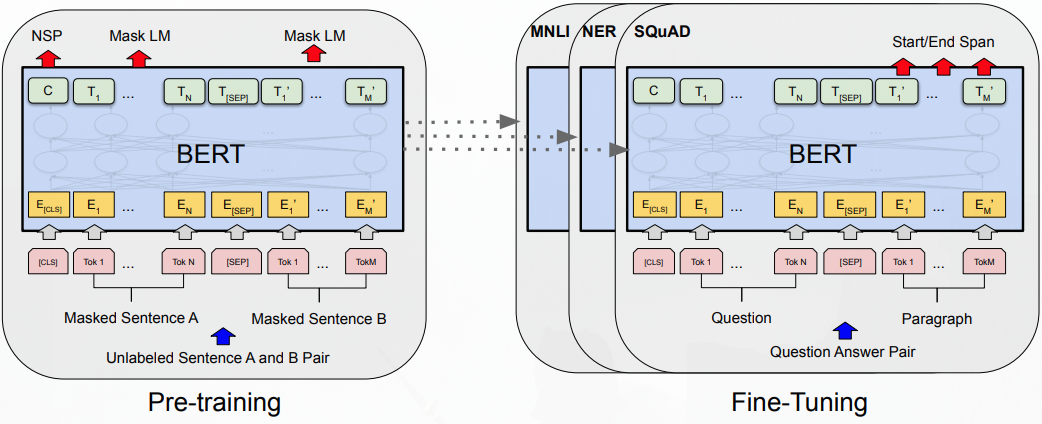
\includegraphics[width=0.95\textwidth]{BERT1.png}
    \caption{The overall pre-training and fine-tuning phases for BERT. For different down-stream tasks, notice the same architecture, except output layer, is used. Source: (\citet{devlin2019bert}).}\label{fig:bert1}
\end{figure}

The pre-training phase can be split into two further training tasks:
\begin{itemize}
    \item  Masked Language Model - During training, a portion of the input tokens are `masked' and the model predicts these masked tokens based on the remaining context, using cross-entropy loss. In the literature, this is referred to as a Cloze task \cite{taylor1953cloze}. In the experiments conducted by (\citet{devlin2019bert}) 15\% of tokens in each sequence are randomly selected for masking. However, to mitigate the mismatch between pre-training and fine-tuning phases, a training data generator replaces each chosen masked tokens with: (1) the special token \texttt{[MASK]} 80\% of the time; (2) a random token 10\% of the time; and (3) the original token itself 10\% of the time.
    \item Next Sentence Prediction - In this task, the model is trained on a binary classification task prediction the relationship between sentence pairs. Given two sentences \texttt{A} and \texttt{B} either (1) sentence \texttt{B} is the actual sentence that follows \texttt{A} 50\% of the time or (2) sentence \texttt{B} is randomly selected from the corpus 50\% of the time. 
\end{itemize}

\subsubsection{XLNet}
\subsubsection{MPNet}
\subsubsection{Nomic}\label{sec:nomic}

\section{Dimensionality Reduction}\label{sec:dimred}
\subsection{PCA}
\subsection{UMAP}

\section{Clustering}
\subsection{k-Medoids}
\subsection{DBSCAN}
\subsection{HDBSCAN}

\section{Clustering Evaluation}
\subsection{Inertia}
\subsection{Silhouette}
\subsection{Davies-Bouldin Index}
\subsection{Calinski-Harabasz Index}

\section{Maybe Optuna}

\clearpage
\chapter{Automatic Label Generation}\label{chap:Methodology}

% \todo[inline,caption={}]{
%     Describe the methods and procedures used.
%     The things in this section will include.
%     \begin{itemize}
%         \item Explaining data format and data visualisation: wordcloud.
%         \item Data cleaning steps, including removing key words such as Ion Source.
%         \item Text preprocessing steps (cleaning) and computational challenges (tensorflow).
%         \item Choosing the best sentence embedding transformer: MPNET, NOMIC.
%         \item Data visualisation (before and after sentence embedding): similarity visualisation, explain unique sentences, token length distribution.
%         \item Motivate why clustering in higher dimensions performs worse
%         \item UMAP, PCA, t-SNE comparison. Motivate using UMAP.
%         \item UMAP hyperparameter optimisation.
%         \item Performing clustering with kmedoids, dbscan, hdbscan.
%         \item Using optuna.
%         \item Evaluation of results and choosing the best model (and arguing why hdbscan is the best by looking at the variance of dbscan and inflexibility of kmedoids)
%         \item Touch on the production of a CLI application that allows you to mix and match various parts of the pipeline. Motivate the need for command line tool.
%     \end{itemize}
% }

\chapter{Results and Discussion}

% \todo[inline,caption={}]{
% Describe the results and analyse the results
% \begin{itemize}
%     \item Analyse the word cloud.
%     \item Analyse the sentence embedding results.
%     \item Analyse UMAP vs. PCA vs. t-SNE qualitatively and later quantitatively (compared to the clustering).
%     \item Anaylse the UMAP hyperparameter optimisation qualitatively, mention that we use Optuna.
% \end{itemize}
% }

\chapter{Conclusion}

% \todo[inline,caption={}]{
% Summarize your findings and suggest areas for future work.
% }

% -------------------------
% References
% -------------------------
% \bibliographystyle{plainnat}

\bibliographystyle{plainnat}
\bibliography{refs}  % Uses the external file refs.bib

\end{document}
